



\documentclass[11pt]{article}

% Language setting
\usepackage[turkish]{babel}
\usepackage{pythonhighlight}

\usepackage[a4paper,top=2cm,bottom=2cm,left=2cm,right=2cm,marginparwidth=2cm]{geometry}

% Useful packages

\usepackage{amsmath}
\usepackage{graphicx}
\usepackage[colorlinks=true, allcolors=blue]{hyperref}
\usepackage{verbatim}
\usepackage{fancyhdr} % for header and footer
\usepackage{titlesec}
\usepackage{parskip}

\setlength{\parindent}{0pt}

\titleformat{\subsection}[runin]{\bfseries}{\thesubsection}{1em}{}

\pagestyle{fancy} % activate the custom header/footer

% define the header/footer contents
\lhead{\small{23BLM-4014 Yapay Sinir Ağları Ara Sınav Soru ve Cevap Kağıdı}}
\rhead{\small{Dr. Ulya Bayram}}
\lfoot{}
\rfoot{}

% remove header/footer on first page
\fancypagestyle{firstpage}{
  \lhead{}
  \rhead{}
  \lfoot{}
  \rfoot{\thepage}
}

\title{Çanakkale Onsekiz Mart Üniversitesi, Mühendislik Fakültesi, Bilgisayar Mühendisliği Akademik Dönem 2022-2023\\
Ders: BLM-4014 Yapay Sinir Ağları/Bahar Dönemi\\ 
ARA SINAV SORU VE CEVAP KAĞIDI\\
Dersi Veren Öğretim Elemanı: Dr. Öğretim Üyesi Ulya Bayram}
\author{%
\begin{minipage}{\textwidth}
\raggedright
Öğrenci Adı Soyadı:  \textbf{Mustafa Beyazbulut}\\ % Adınızı soyadınızı ve öğrenci numaranızı noktaların yerine yazın
Öğrenci No:  \textbf{190401085}
\end{minipage}%
}

\date{14 Nisan 2023}

\begin{document}
\maketitle

\vspace{-.5in}
\section*{Açıklamalar:}
\begin{itemize}
    \item Vizeyi çözüp, üzerinde aynı sorular, sizin cevaplar ve sonuçlar olan versiyonunu bu formatta PDF olarak, Teams üzerinden açtığım assignment kısmına yüklemeniz gerekiyor. Bu bahsi geçen PDF'i oluşturmak için LaTeX kullandıysanız, tex dosyasının da yer aldığı Github linkini de ödevin en başına (aşağı url olarak) eklerseniz bonus 5 Puan! (Tavsiye: Overleaf)
    \item Çözümlerde ya da çözümlerin kontrolünü yapmada internetten faydalanmak, ChatGPT gibi servisleri kullanmak serbest. Fakat, herkesin çözümü kendi emeğinden oluşmak zorunda. Çözümlerinizi, cevaplarınızı aşağıda belirttiğim tarih ve saate kadar kimseyle paylaşmayınız. 
    \item Kopyayı önlemek için Github repository'lerinizin hiçbirini \textbf{14 Nisan 2023, saat 15:00'a kadar halka açık (public) yapmayınız!} (Assignment son yükleme saati 13:00 ama internet bağlantısı sorunları olabilir diye en fazla ekstra 2 saat daha vaktiniz var. \textbf{Fakat 13:00 - 15:00 arası yüklemelerden -5 puan!}
    \item Ek puan almak için sağlayacağınız tüm Github repository'lerini \textbf{en geç 15 Nisan 2023 15:00'da halka açık (public) yapmış olun linklerden puan alabilmek için!}
    \item \textbf{14 Nisan 2023, saat 15:00'dan sonra gönderilen vizeler değerlendirilmeye alınmayacak, vize notu olarak 0 (sıfır) verilecektir!} Son anda internet bağlantısı gibi sebeplerden sıfır almayı önlemek için assignment kısmından ara ara çözümlerinizi yükleyebilirsiniz yedekleme için. Verilen son tarih/saatte (14 Nisan 2023, saat 15:00) sistemdeki en son yüklü PDF geçerli olacak.
    \item Çözümlerin ve kodların size ait ve özgün olup olmadığını kontrol eden bir algoritma kullanılacaktır. Kopya çektiği belirlenen vizeler otomatikman 0 (sıfır) alacaktır. Bu nedenle çözümlerinizi ve kodlarınızı yukarıda sağladığım gün ve saatlere kadar kimseyle paylaşmayınız.
    \item Bu vizeden alınabilecek en yüksek not 100'dür. Toplam aldığınız puan 100'ü geçerse, aldığınız not 100'e sabitlenecektir.
    \item LaTeX kullanarak PDF oluşturanlar öz geçmişlerine LaTeX bildiklerini de eklemeyi unutmasınlar :)
    \item Bu vizedeki soruların çözümleri ve tex dosyası için istediğiniz kadar sayıda Github repository'si oluşturabilirsiniz. Sadece yukarıda belirttiğim tarihlerde (14 Nisan 2023 saat 15:00 ile 15 Nisan 2023 saat 15:00 arasında) public yapmayı/halka açmayı ve Github profilinizi de öz geçmişinize eklemeyi unutmayın :)
    \item Bilgisayarınıza hiçbir program kurmadan, Overleaf, Google Colab, Kaggle gibi ortamlar üzerinden bu vizeyi tamamlamanız mümkün. İyi çalışmalar!!
\end{itemize}
(5p) \url{https://github.com/mustafabeyazbulut/Python/blob/main/Yapay_Sinir_Aglari/main.tex}

\newpage
\section{(Toplam 10 Puan) Hopfield Networks:}

\subsection{(2 Puan)} \textbf{ChatGPT’ye size Hopfield Network’ler ile ilgili detaylı bilgi vermesini isteyin. Sorduğunuz soruyu, ChatGPT'nin çıkartığı cevabı aşağı koyun. Bu cevapta anlamadığınız terimleri de ChatGPT’ye sorup, sorduğunuz soruları ve ChatGPT’nin verdiği cevapları da sırayla aşağı koyun.}

“Hopfield Network" Hakkında detaylı bilgi verebilir misin?

Hopfield ağı, bellek ve assoziatif hatırlama işlemlerinde kullanılan bir yapay sinir ağı modelidir. Bu ağ, bağlantıları tek yönlü olmayan bir sinir ağıdır ve tüm düğümler diğer tüm düğümlere bağlıdır. Bu bağlantıların ağırlıkları, Hopfield ağına özgü olan bir öğrenme kuralı kullanılarak belirlenir.

Hopfield ağı, basitçe, birçok nöronun birbirleriyle bağlı olduğu bir ağdır. Her nöron, diğer nöronlara bir çıkış sinyali üretir ve aynı zamanda diğer nöronlardan gelen sinyalleri alır. Bu sinyallerin toplamı, her nöronun bir çıkış sinyali üretmesini sağlar.

Hopfield ağı, assoziatif bellek işlemleri için kullanılabilir. Assoziatif bellek, bir şeyi hatırlamak için onunla ilgili anahtar kelimeyi hatırlama işlemidir. Örneğin, "elma" kelimesini hatırlamak için, elmanın şekli, rengi, tadı gibi özellikleri hatırlanır. Hopfield ağı, bu tür bellek işlemlerinde kullanılan bir yöntemdir. Öğrenme işlemi sırasında, ağa öğrenilecek örnekler verilir ve ağ bu örnekleri belleğinde saklar. Daha sonra, anahtar kelimeyi girdi olarak verdiğinizde, ağ, anahtar kelime ile en çok ilişkili örneği hatırlar ve çıkış olarak verir.

Hopfield ağı, diğer yapay sinir ağı modellerinden farklı olarak, enerji fonksiyonu olarak adlandırılan bir matematiksel fonksiyonu kullanır. Enerji fonksiyonu, ağın içinde bulunduğu durumun enerjisini belirler ve ağın durumunu değiştirmek için kullanılır.

Hopfield ağının bir diğer özelliği, ağın her zaman bir sabit duruma yakınsamasıdır. Bu durum, ağın bir çıkış sinyali ürettiği ve artık değişmediği durumdur. Bu özellik, ağın durağan bir şekilde çalışmasını sağlar.

Hopfield ağı, birçok alanda kullanılabilir. Örneğin, optik karakter tanıma, sinyal işleme, robotik, biyoinformatik gibi alanlarda kullanılabilir.


\subsection{(8 Puan)} \textbf{ChatGPT’nin açıklamalarından ne anladığınızı buraya kendi kelimelerinizle özetleyin. Örneğin ``Hopfield Network nedir? Ne işe yarar? Neden bilmemiz gerekir bunu? Gerçek hayatta kullanılıyor mu?'' gibi. Anlamadığınız kısımlar varsa ve ChatGPT’nin açıklamaları yeterli gelmezse internet dahil farklı kaynaklardan araştırıp, bilgilerin doğruluğunu sorgulamakta serbestsiniz. Konuyu doğru anlayıp anlamamanız puana etki edecektir. Kullandığınız kaynakları da belirtin!}

Hopfield Network nedir?

Hopfield Network, insan hafızası gibi çalışması amaçlanan bir yapay sinir ağıdır. uygulamalarda da kullanılabilir.

Ne işe yarar?

Bu, bellek içinde bir anahtar kelime verildiğinde, ağın önceden öğrendiği örnekler arasından en uygun olanını hatırlamasını sağlar.Bunun yanı sıra, Hopfield ağları, en az enerji gerektiren hedef fonksiyonunu belirleyerek, optimize etme ve veri sıkıştırma gibi diğer 

Neden bilmemiz gerekir bunu?

Bu nedenle, makine öğrenimi, yapay zeka ve sınıflandırma problemlerinin çözümünde kullanılan diğer tekniklerle birlikte öğrenilmesi gereken önemli bir konudur. Bununla birlikte, günümüzde gerçek hayatta kullanımı sınırlıdır.

Gerçek hayatta kullanılıyor mu?

Evet, Hopfield ağları gerçek hayatta birçok alanda kullanılır. Örneğin, mühendislikte, enerji yönetiminde, robotikte, tıpta ve bilgisayar bilimlerinde kullanılır. Hopfield ağları ayrıca, hafıza işlemleri, tanıma işlemleri ve optimizasyon problemleri gibi birçok alanda da kullanılır. Örneğin, bir Hopfield ağı, yüz tanıma gibi bir görüntü işleme uygulamasında kullanılabilir veya iş sıralama gibi bir optimizasyon problemi için de kullanılabilir.

\section{(Toplam 10 Puan) Boltzman Machine:}

\subsection{(2 Puan)} \textbf{ChatGPT’ye size Boltzman Machine ilgili detaylı bilgi vermesini isteyin. Sorduğunuz soruyu, ChatGPT'nin çıkartığı cevabı aşağı koyun. Bu cevapta anlamadığınız terimleri de ChatGPT’ye sorup, sorduğunuz soruları ve ChatGPT’nin verdiği cevapları da sırayla aşağı koyun.}

“Boltzman Machine" Hakkında detaylı bilgi verebilir misin?

Boltzmann Machine, yapay sinir ağlarından bir tür olup, öğrenme algoritması aracılığıyla öğrenme yapabilen bir tür yapay sinir ağıdır. Bu makine, çıktılarına bağlı olmayan gizli katmanlar içerir ve bu katmanlar, giriş verilerinin özniteliklerini öğrenmek için kullanılır.

Bir Boltzmann Machine, enerji fonksiyonu olarak adlandırılan bir fonksiyon kullanır ve bu fonksiyon, ağın mevcut durumundaki bir enerji seviyesini belirler. Bu enerji seviyesi, ağın belirli bir durumda kalma olasılığına karşılık gelir. Ağ, bir veri noktasıyla eşleştirildiğinde, ağın enerji seviyesi düşürülür ve bu da ağın giriş verilerine benzer verileri daha olası hale getirir.

Boltzmann Machine, çift yönlü bağlantıları olan bir yapay sinir ağıdır. Bu özelliği nedeniyle, Boltzmann Machine, giriş verilerindeki öznitelikleri öğrenmek için kullanılır. Ağın giriş verilerine bağlı olarak, ağın gizli katmanındaki bir nöronun aktive olma olasılığı artar. Bu nöronun aktive olması, ağın başka bir nöronunda da bir aktive olma olasılığını arttırır ve bu nöronların etkileşimi, giriş verilerindeki özniteliklerin öğrenilmesine yardımcı olur.

Boltzmann Machine, birçok farklı öğrenme algoritması kullanarak eğitilebilir. Ancak, en yaygın olarak kullanılan öğrenme algoritması, çekimli öğrenme olarak adlandırılan bir yöntemdir. Bu algoritma, ağın enerji seviyesini azaltmak için giriş verileriyle çalışır ve ağı giriş verilerine benzer verileri daha olası hale getirir.

Boltzmann Machine, birçok uygulamada kullanılmaktadır. Özellikle, görüntü tanıma, doğal dil işleme, sınıflandırma ve benzeri alanlarda kullanılmaktadır.

\subsection{(8 Puan)} \textbf{ChatGPT’nin açıklamalarından ne anladığınızı buraya kendi kelimelerinizle özetleyin. Örneğin ``Boltzman Machine nedir? Ne işe yarar? Neden bilmemiz gerekir bunu? Gerçek hayatta kullanılıyor mu?'' gibi. Anlamadığınız kısımlar varsa ve ChatGPT’nin açıklamaları yeterli gelmezse internet dahil farklı kaynaklardan araştırıp, bilgilerin doğruluğunu sorgulamakta serbestsiniz. Konuyu doğru anlayıp anlamamanız puana etki edecektir. Kullandığınız kaynakları da belirtin!}

Boltzman Machine nedir?

Boltzman Machine, giriş veri seti üzerinden öğrenme işlemi gerçekleştirir. Boltzman Machine de görünür ve gizli olmak üzere iki katmanlı bir yapıya sahip olduğu anlaşılmaktadır.

Ne işe yarar?

Boltzmann Machine, yapay sinir ağlarının bir türüdür ve öğrenme algoritmaları için kullanılır. Hesaplama açısından çok güçlüdür ve özellikle sinir ağı yapısının karmaşık olduğu durumlarda kullanılır. Boltzmann Machine, girdileri öğrenerek bir çıktı üretir ve bu çıktı, girdilerin belirli bir kalıbını tanımak için kullanılabilir.

Neden bilmemiz gerekir bunu?

Makine öğrenmesi alanındaki ileri düzey uygulamalarda sıklıkla kullanılmaktadır ve bu nedenle bu algoritmayı bilmek, yapay zeka ve makine öğrenmesi konularında ileri düzey bilgi sahibi olmak isteyenler için önemlidir

Gerçek hayatta kullanılıyor mu?

Özellikle makine öğrenimi, yapay zeka ve veri analizi gibi alanlarda kullanılmıştır. Örneğin, yüz tanıma, nesne tanıma, dil modellemesi ve öneri sistemleri gibi birçok alanda Boltzmann Machine kullanılmıştır. Ayrıca, enerji yönetimi, finansal tahminler ve tıbbi teşhis gibi diğer uygulamalarda da kullanılabilir. Ancak, diğer yapay sinir ağı modelleri daha popüler hale gelmiştir ve Boltzmann Machine, diğer modellerle karşılaştırıldığında daha az kullanılmaktadır

\section{(Toplam 10 Puan) Markov Assumption ve Markov Chain:}

\subsection{(2 Puan)} \textbf{ChatGPT’ye size Markov assumption ve Markov Chain ilgili detaylı bilgi vermesini isteyin. Sorduğunuz soruyu, ChatGPT'nin çıkartığı cevabı aşağı koyun. Bu cevapta anlamadığınız terimleri de ChatGPT’ye sorup, sorduğunuz soruları ve ChatGPT’nin verdiği cevapları da sırayla aşağı koyun.}

Markov assumption ve Markov Chain ile ilgili detaylı bilgi verebilir misin 

Elbette! Markov Assumption (Markov Varsayımı) ve Markov Zinciri (Markov Chain), olasılık teorisi ve istatistiklerde kullanılan bir kavramdır.

Markov Assumption, bir süreçte (genellikle zamanla değişen bir süreçte) bir sonraki durumun, sadece mevcut duruma bağlı olduğunu ve geçmiş durumlardan bağımsız olduğunu varsayar. Başka bir deyişle, bir sürecin gelecekteki durumu, yalnızca şu anki durumuna bağlıdır ve geçmiş durumları göz önünde bulundurmaz. Bu varsayım, birçok gerçek dünya sürecinin modellenmesinde kullanılır ve çeşitli uygulamalarda, özellikle zaman serileri analizinde ve doğal dil işleme problemlerinde kullanılır.

Markov Zinciri, Markov Assumption'a dayanan bir olasılık süreçtir. Bir Markov Zinciri, bir dizi durumun oluşturduğu bir süreçtir ve her bir durumun oluşma olasılığı, yalnızca bir önceki duruma bağlıdır. Yani, bir Markov Zinciri, bir sürecin herhangi bir anındaki durumunu, yalnızca bir önceki durumunun bilgisine dayanarak tahmin eder.

Formal olarak, bir Markov Zinciri, aşağıdaki iki özelliğe sahip bir olasılık süreçtir:

Markov Property: Bir sürecin herhangi bir anındaki durumu, sadece bir önceki durumunun bilgisine bağlıdır. Geçmiş durumlar, gelecekteki durumları tahmin etmede etkili değildir.

Geçiş Olasılıkları: Herhangi iki durum arasındaki geçiş olasılıkları bellidir ve zamanla değişmezdir. Yani, bir durumun bir sonraki duruma geçme olasılığı, süreçteki zaman adımına bağlı değildir.

Markov Zincirleri, birçok uygulamada kullanılır. Özellikle, rastgele olayların modellemesi, zaman serileri analizi, stokastik süreçlerin modellenmesi, hava durumu tahminleri, finansal piyasa modelleri, doğal dil işleme ve daha pek çok alanda kullanılır. Markov Zincirleri, süreçlerin davranışını modellemek, tahmin yapmak, olasılık dağılımlarını hesaplamak ve diğer birçok analiz yapmak için kullanılabilir. Ayrıca, Markov Zincirleri, Markov Rastgele Alan Modelleri (Markov Random Field) ve Gizli Markov Modelleri (Hidden Markov Models) gibi daha karmaşık modellere temel oluşturabilir.

\subsection{(8 Puan)} \textbf{ChatGPT’nin açıklamalarından ne anladığınızı buraya kendi kelimelerinizle özetleyin. Örneğin ``Markov assumption ve Markov Chain nedir? Ne işe yarar? Neden bilmemiz gerekir bunu? Gerçek hayatta kullanılıyor mu?'' gibi. Anlamadığınız kısımlar varsa ve ChatGPT’nin açıklamaları yeterli gelmezse internet dahil farklı kaynaklardan araştırıp, bilgilerin doğruluğunu sorgulamakta serbestsiniz. Konuyu doğru anlayıp anlamamanız puana etki edecektir. Kullandığınız kaynakları da belirtin!}

Markov Assumption, bir süreçte bir sonraki durumun mevcut duruma bağlı olduğunu savunur yani gelecekteki durum şu anki duruma bağlıdır. Geçmişte ki durumlarla ilgilenmez. Gerçek dünya süreçlerinin modellenmesinde kullanılır. Örnek olarak doğal dil işlemede kullanılır.

Markov zinciri de Markov Assumption'a dayanır. Bir olasılık sürecidir. Burada da her bir durumun oluşma olasılığı mevcut duruma bağlıdır. Yani, bir Markov Zinciri, bir sürecin herhangi bir anındaki durumunu, yalnızca bir önceki durumunun bilgisine dayanarak tahmin eder. iki özelliğe sahiptir. Bunlar Markov Property ve Geçiş olasılıklarıdır.


\section{(Toplam 20 Puan) Feed Forward:}
 
\begin{itemize}
    \item Forward propagation için, input olarak şu X matrisini verin (tensöre çevirmeyi unutmayın):\\
    $X = \begin{bmatrix}
        1 & 2 & 3\\
        4 & 5 & 6
        \end{bmatrix}$
    Satırlar veriler (sample'lar), kolonlar öznitelikler (feature'lar).
    \item Bir adet hidden layer olsun ve içinde tanh aktivasyon fonksiyonu olsun
    \item Hidden layer'da 50 nöron olsun
    \item Bir adet output layer olsun, tek nöronu olsun ve içinde sigmoid aktivasyon fonksiyonu olsun
\end{itemize}

\begin{comment}
Tanh fonksiyonu:\\
$f(x) = \frac{exp(x) - exp(-x)}{exp(x) + exp(-x)}$
\vspace{.2in}

Sigmoid fonksiyonu:\\
$f(x) = \frac{1}{1 + exp(-x)}$
\end{comment}

\begin{align*}
& \text{Tanh fonksiyonu: } f(x) = \frac{\exp(x) - \exp(-x)}{\exp(x) + \exp(-x)} \
& \text{Sigmoid fonksiyonu: } f(x) = \frac{1}{1 + \exp(-x)}
\end{align*}


 \textbf{Pytorch kütüphanesi ile, ama kütüphanenin hazır aktivasyon fonksiyonlarını kullanmadan, formülünü verdiğim iki aktivasyon fonksiyonunun kodunu ikinci haftada yaptığımız gibi kendiniz yazarak bu yapay sinir ağını oluşturun ve aşağıdaki üç soruya cevap verin.}
 
\subsection{(10 Puan)} \textbf{Yukarıdaki yapay sinir ağını çalıştırmadan önce pytorch için Seed değerini 1 olarak set edin, kodu aşağıdaki kod bloğuna ve altına da sonucu yapıştırın:}

% Latex'de kod koyabilirsiniz python formatında. Aşağıdaki örnekleri silip içine kendi kodunuzu koyun
\begin{python}
import torch
import torch.nn as nn
seed=1
torch.manual_seed(seed=seed)
x = torch.tensor([[1, 2, 3], [4, 5, 6]], dtype=torch.float32)

class FeedForward(nn.Module):
    def __init__(self):
        super(FeedForward, self).__init__()
        self.hidden_layer = nn.Linear(3, 50)
        self.output_layer = nn.Linear(50, 1)

    def forward(self, x):
        x = self.tanh_activation(self.hidden_layer(x))
        x = self.sigmoid_activation(self.output_layer(x))
        return x
    
    def tanh_activation(self, x):
        return (torch.exp(x) - torch.exp(-x)) / (torch.exp(x) + torch.exp(-x))
    
    def sigmoid_activation(self, x):
        return 1 / (1 + torch.exp(-x))

model = FeedForward()
output = model(x)

print('seed degeri:' , seed, ' output degeri:' ,  output.data)
\end{python}

 \textbf{seed degeri:} 1   \textbf{output degeri:}  tensor([[0.4892], [0.5566]])

\subsection{(5 Puan)} \textbf{Yukarıdaki yapay sinir ağını çalıştırmadan önce Seed değerini öğrenci numaranız olarak değiştirip, kodu aşağıdaki kod bloğuna ve altına da sonucu yapıştırın:}
\vspace{.6in}

\begin{python}
import torch
import torch.nn as nn

seed=190401085
torch.manual_seed(seed=seed)

x = torch.tensor([[1, 2, 3], [4, 5, 6]], dtype=torch.float32)

class FeedForward(nn.Module):
    def __init__(self):
        super(FeedForward, self).__init__()
        self.hidden_layer = nn.Linear(3, 50)
        self.output_layer = nn.Linear(50, 1)

    def forward(self, x):
        x = self.tanh_activation(self.hidden_layer(x))
        x = self.sigmoid_activation(self.output_layer(x))
        return x
    
    def tanh_activation(self, x):
        return (torch.exp(x) - torch.exp(-x)) / (torch.exp(x) + torch.exp(-x))
    
    def sigmoid_activation(self, x):
        return 1 / (1 + torch.exp(-x))

model = FeedForward()
output = model(x)



print('seed degeri:' , seed, ' output degeri:' ,  output.data)
\end{python}

\vspace{.2in}

 \textbf{seed degeri:} 190401085   \textbf{output degeri:} tensor([[0.4991], [0.4573]])

\vspace{.6in}
\subsection{(5 Puan)} \textbf{Kodlarınızın ve sonuçlarınızın olduğu jupyter notebook'un Github repository'sindeki linkini aşağıdaki url kısmının içine yapıştırın. İlk sayfada belirttiğim gün ve saate kadar halka açık (public) olmasın:}
% size ait Github olmak zorunda, bu vize için ayrı bir github repository'si açıp notebook'u onun içine koyun. Kendine ait olmayıp da arkadaşının notebook'unun linkini paylaşanlar 0 alacak.

\vspace{.2in}
\url{https://github.com/mustafabeyazbulut/Python/blob/main/Yapay_Sinir_Aglari/FeedForward/Feed_Forward.ipynb}

\newpage
\section{(Toplam 40 Puan) Multilayer Perceptron (MLP):} 
\textbf{Bu bölümdeki sorularda benim vize ile beraber paylaştığım Prensesi İyileştir (Cure The Princess) Veri Seti parçaları kullanılacak. Hikaye şöyle (soruyu çözmek için hikaye kısmını okumak zorunda değilsiniz):} 

``Bir zamanlar, çok uzaklarda bir ülkede, ağır bir hastalığa yakalanmış bir prenses yaşarmış. Ülkenin kralı ve kraliçesi onu iyileştirmek için ellerinden gelen her şeyi yapmışlar, ancak denedikleri hiçbir çare işe yaramamış.

Yerel bir grup köylü, herhangi bir hastalığı iyileştirmek için gücü olduğu söylenen bir dizi sihirli malzemeden bahsederek kral ve kraliçeye yaklaşmış. Ancak, köylüler kral ile kraliçeyi, bu malzemelerin etkilerinin patlayıcı olabileceği ve son zamanlarda yaşanan kuraklıklar nedeniyle bu malzemelerden sadece birkaçının herhangi bir zamanda bulunabileceği konusunda uyarmışlar. Ayrıca, sadece deneyimli bir simyacı bu özelliklere sahip patlayıcı ve az bulunan malzemelerin belirli bir kombinasyonunun prensesi iyileştireceğini belirleyebilecekmiş.

Kral ve kraliçe kızlarını kurtarmak için umutsuzlar, bu yüzden ülkedeki en iyi simyacıyı bulmak için yola çıkmışlar. Dağları tepeleri aşmışlar ve nihayet "Yapay Sinir Ağları Uzmanı" olarak bilinen yeni bir sihirli sanatın ustası olarak ün yapmış bir simyacı bulmuşlar.

Simyacı önce köylülerin iddialarını ve her bir malzemenin alınan miktarlarını, ayrıca iyileşmeye yol açıp açmadığını incelemiş. Simyacı biliyormuş ki bu prensesi iyileştirmek için tek bir şansı varmış ve bunu doğru yapmak zorundaymış. (Original source: \url{https://www.kaggle.com/datasets/unmoved/cure-the-princess})

(Buradan itibaren ChatGPT ve Dr. Ulya Bayram'a ait hikayenin devamı)

Simyacı, büyülü bileşenlerin farklı kombinasyonlarını analiz etmek ve denemek için günler harcamış. Sonunda birkaç denemenin ardından prensesi iyileştirecek çeşitli karışım kombinasyonları bulmuş ve bunları bir veri setinde toplamış. Daha sonra bu veri setini eğitim, validasyon ve test setleri olarak üç parçaya ayırmış ve bunun üzerinde bir yapay sinir ağı eğiterek kendi yöntemi ile prensesi iyileştirme ihtimalini hesaplamış ve ikna olunca kral ve kraliçeye haber vermiş. Heyecanlı ve umutlu olan kral ve kraliçe, simyacının prensese hazırladığı ilacı vermesine izin vermiş ve ilaç işe yaramış ve prenses hastalığından kurtulmuş.

Kral ve kraliçe, kızlarının hayatını kurtardığı için simyacıya krallıkta kalması ve çalışmalarına devam etmesi için büyük bir araştırma bütçesi ve çok sayıda GPU'su olan bir server vermiş. İyileşen prenses de kendisini iyileştiren yöntemleri öğrenmeye merak salıp, krallıktaki üniversitenin bilgisayar mühendisliği bölümüne girmiş ve mezun olur olmaz da simyacının yanında, onun araştırma grubunda çalışmaya başlamış. Uzun yıllar birlikte krallıktaki insanlara, hayvanlara ve doğaya faydalı olacak yazılımlar geliştirmişler, ve simyacı emekli olduğunda prenses hem araştırma grubunun hem de krallığın lideri olarak hayatına devam etmiş.

Prenses, kendisini iyileştiren veri setini de, gelecekte onların izinden gidecek bilgisayar mühendisi prensler ve prensesler başkalarına faydalı olabilecek yapay sinir ağları oluşturmayı öğrensinler diye halka açmış ve sınavlarda kullanılmasını salık vermiş.''

\textbf{İki hidden layer'lı bir Multilayer Perceptron (MLP) oluşturun beşinci ve altıncı haftalarda yaptığımız gibi. Hazır aktivasyon fonksiyonlarını kullanmak serbest. İlk hidden layer'da 100, ikinci hidden layer'da 50 nöron olsun. Hidden layer'larda ReLU, output layer'da sigmoid aktivasyonu olsun.}

\textbf{Output layer'da kaç nöron olacağını veri setinden bakıp bulacaksınız. Elbette bu veriye uygun Cross Entropy loss yöntemini uygulayacaksınız. Optimizasyon için Stochastic Gradient Descent yeterli. Epoch sayınızı ve learning rate'i validasyon seti üzerinde denemeler yaparak (loss'lara overfit var mı diye bakarak) kendiniz belirleyeceksiniz. Batch size'ı 16 seçebilirsiniz.}
\newpage

\subsection{(10 Puan)} \textbf{Bu MLP'nin pytorch ile yazılmış class'ının kodunu aşağı kod bloğuna yapıştırın:}
\vspace{.3in}
\begin{python}
#Model olusturuyoruz
import torch.nn as nn

class MLP(nn.Module):
    def __init__(self, input_size, hidden_size1, hidden_size2, output_size):
        super(MLP, self).__init__()
        self.fc1 = nn.Linear(input_size, hidden_size1)
        self.fc2 = nn.Linear(hidden_size1, hidden_size2)
        self.fc3 = nn.Linear(hidden_size2, output_size)
        self.relu = nn.ReLU()
        self.sigmoid = nn.Sigmoid()

    def forward(self, x):
        out = self.fc1(x)
        out = self.relu(out)
        out = self.fc2(out)
        out = self.relu(out)
        out = self.fc3(out)
        out = self.sigmoid(out)
        return out
\end{python}
\vspace{.5in}
\subsection{(10 Puan)} \textbf{SEED=öğrenci numaranız set ettikten sonra altıncı haftada yazdığımız gibi training batch'lerinden eğitim loss'ları, validation batch'lerinden validasyon loss değerlerini hesaplayan kodu aşağıdaki kod bloğuna yapıştırın ve çıkan figürü de alta ekleyin.}
\vspace{.3in}
\begin{python}
torch.manual_seed(190401085)
train_loss_list = [] # train loss listesi
val_loss_list = [] # validation loss listesi

num_epochs = 50

# Her bir epoch'ta dongu
for epoch in range(num_epochs):
    # Model egitim modunda (training mode) olacak
    model.train()
    train_loss = 0
    train_correct = 0
    train_total = 0

    # Her bir batch (yigin) icin dongu
    for i, (inputs, labels) in enumerate(train_loader):
        # Verileri GPU'ya tasi
        inputs, labels = inputs.to(device), labels.to(device)

        # Gradientleri sifirla
        optimizer.zero_grad()

        # Forward pass islemi
        outputs = model(inputs)

        # Loss hesapla
        loss = criterion(outputs, labels)

        # Gradientleri backward islemi ile hesapla
        loss.backward()

        # Optimize etmek icin weights (agirliklar) guncelle
        optimizer.step()

        # Toplam loss degerini ve dogru tahmin sayisini guncelle
        train_loss += loss.item() * inputs.size(0)
        _, predicted = torch.max(outputs.data, 1)
        train_total += labels.size(0)
        train_correct += (predicted == labels).sum().item()

        # Her 100 batchte bir kaybi yazdir
        if (i+1) % 100 == 0:
            print(f'Epoch [{epoch+1}/{num_epochs}], Step [{i+1}/{len(train_loader)}], Loss: {loss.item():.4f}')

    # Train loss'un ortalamasini al ve kaydet
    train_loss = train_loss / len(train_loader.dataset)
    train_acc = 100 * train_correct / train_total
    train_loss_list.append(train_loss)

    # Model degerlendirme modunda (evaluation mode) olacak
    model.eval()

    # Validation veri seti uzerinde degerlendirme
    with torch.no_grad():
        val_loss = 0
        val_correct = 0
        val_total = 0

        # Her bir batch (yigin) icin dongu
        for inputs, labels in val_loader:
        
            # Verileri GPU'ya tasi
            inputs, labels = inputs.to(device), labels.to(device)
            
            # Forward pass islemi
            outputs = model(inputs)
            
            # Loss hesapla
            loss = criterion(outputs, labels)

            # Toplam loss degerini ve dogru tahmin sayisini guncelle
            val_loss += loss.item() * inputs.size(0)
            _, predicted = torch.max(outputs.data, 1)
            val_total += labels.size(0)
            val_correct += (predicted == labels).sum().item()
            
        # Validation loss'un ortalamasini al ve kaydet
        val_loss = val_loss / len(val_loader.dataset)
        val_acc = 100 * val_correct / val_total
        val_loss_list.append(val_loss)
        
    # Her epoch sonunda train loss, train accuracy, validation loss ve validation accuracy'yi yazdir
    print(f'Epoch: {epoch+1}/{num_epochs} - Train Loss: {train_loss:.4f} - Train Acc: {train_acc:.2f}% - Val Loss: {val_loss:.4f} - Val Acc: {val_acc:.2f}% ')
\end{python}

\newpage
\vspace{.3in}
\begin{figure}[ht!]
    \centering
    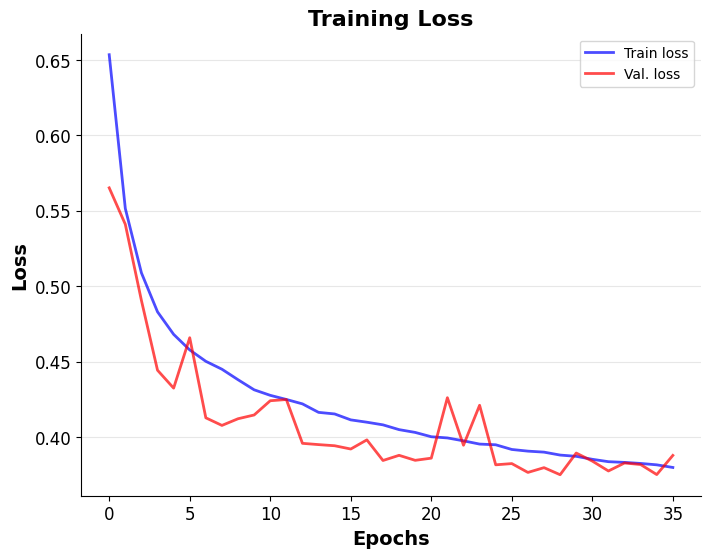
\includegraphics[]{figure5_1.png}
    \caption{Train and Validation Losses}
    \label{fig:my_pic}
\end{figure}


\vspace{.6in}
\subsection{(10 Puan)} \textbf{SEED=öğrenci numaranız set ettikten sonra altıncı haftada ödev olarak verdiğim gibi earlystopping'deki en iyi modeli kullanarak, Prensesi İyileştir test setinden accuracy, F1, precision ve recall değerlerini hesaplayan kodu yazın ve sonucu da aşağı yapıştırın. \%80'den fazla başarı bekliyorum test setinden. Daha düşükse başarı oranınız, nerede hata yaptığınızı bulmaya çalışın. \%90'dan fazla başarı almak mümkün (ben denedim).}

\vspace{.3in}

\begin{python}
new_model = MLP(input_size, hidden_size1, hidden_size2, output_size).to(device)

# Kaydedilmis modelin dosya yolunu belirleyin
model_path = '/content/checkpoint.pt'

# En iyi modeli yukleyin
new_model.load_state_dict(torch.load(model_path))

# Yeni modelin performansini degerlendirme modunda (evaluation mode) ayarlayin
new_model.eval()

# Test veri seti degerlendirme
with torch.no_grad():
    predicted_labels = []
    true_labels = []
    for inputs, labels in test_loader:
        inputs, labels = inputs.to(device), labels.to(device)
        outputs = new_model(inputs)
        _, predicted = torch.max(outputs.data, 1)
        predicted_labels += predicted.tolist()
        true_labels += labels.tolist()
        
from sklearn.metrics import accuracy_score, precision_score, recall_score, f1_score

# Sklearn kutuphanesi ile hesaplanan metrik degerleri yazdirma
print("Accuracy: {:.4f}".format(accuracy_score(true_labels, predicted_labels)))
print("Precision: {:.4f}".format(precision_score(true_labels, predicted_labels)))
print("Recall: {:.4f}".format(recall_score(true_labels, predicted_labels)))
print("F1 Score: {:.4f}".format(f1_score(true_labels, predicted_labels)))

\end{python}

\vspace{.3in}

\begin{flushleft}
Accuracy    : 0.9288\\
Precision   : 0.9393\\
Recall      : 0.9175\\
F1 Score    : 0.9283
\end{flushleft}

\vspace{.6in}
\subsection{(5 Puan)} \textbf{Tüm kodların CPU'da çalışması ne kadar sürüyor hesaplayın. Sonra to device yöntemini kullanarak modeli ve verileri GPU'ya atıp kodu bir de böyle çalıştırın ve ne kadar sürdüğünü hesaplayın. Süreleri aşağıdaki tabloya koyun. GPU için Google Colab ya da Kaggle'ı kullanabilirsiniz, iki ortam da her hafta saatlerce GPU hakkı veriyor.}

\vspace{.6in}

\begin{table}[ht!]
    \centering
    \begin{tabular}{c|c}
        Ortam & Süre (saniye) \\\hline
        CPU & 6.448095 \\
        GPU & 15.916516\\
    \end{tabular}
    \label{tab:my_table}
\end{table}

\newpage

\subsection{(3 Puan)} \textbf{Modelin eğitim setine overfit etmesi için elinizden geldiği kadar kodu gereken şekilde değiştirin, validasyon loss'unun açıkça yükselmeye başladığı, training ve validation loss'ları içeren figürü aşağı koyun ve overfit için yaptığınız değişiklikleri aşağı yazın. Overfit, tam bir çanak gibi olmalı ve yükselmeli. Ona göre parametrelerle oynayın.}

Kodlarımda bulunan Dropout , L2 ve Early stopping işlemlerini kaldırdım. Learning rate değerlerini değiştirdim. Veri setini küçülttüm. 
\begin{figure}[ht!]
    \centering
    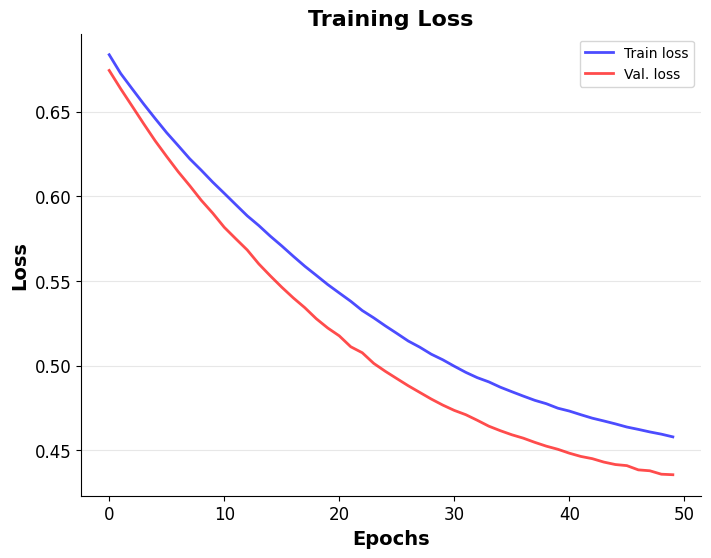
\includegraphics[]{figure5_5.png}
    \caption{Train and Validation Losses}
    \label{fig:my_pic2}
\end{figure}


\subsection{(2 Puan)} \textbf{Beşinci soruya ait tüm kodların ve cevapların olduğu jupyter notebook'un Github linkini aşağıdaki url'e koyun.}

\url{https://github.com/mustafabeyazbulut/Python/tree/main/Yapay_Sinir_Aglari/MultilayerPerceptron(MLP)/MLP1.ipynb}

\newpage

\section{(Toplam 10 Puan)} \textbf{Bir önceki sorudaki Prensesi İyileştir problemindeki yapay sinir ağınıza seçtiğiniz herhangi iki farklı regülarizasyon yöntemi ekleyin ve aşağıdaki soruları cevaplayın.} 



\subsection{(2 puan)} \textbf{Kodlarda regülarizasyon eklediğiniz kısımları aşağı koyun:} 
\vspace{.4in}
\begin{python}
class L2Regularization(nn.Module):
    def __init__(self, weight_decay):
        super(L2Regularization, self).__init__()
        self.weight_decay = weight_decay

    def forward(self, model):
        l2_reg = torch.tensor(0.).to(device)
        for name, param in model.named_parameters():
            if 'weight' in name:
                l2_reg += torch.norm(param, p=2)**2
        return self.weight_decay * l2_reg

class DropoutRegularization(nn.Module):
    def __init__(self, dropout_prob):
        super(DropoutRegularization, self).__init__()
        self.dropout_prob = dropout_prob
        self.dropout = nn.Dropout(p=dropout_prob)

    def forward(self, x):
        x = self.dropout(x)
        return x
\end{python}
\vspace{.2in}
L2 ve Dropout için class oluşturdum. 

\vspace{.4in}
\begin{python}

# Dropout regulasyonu icin DropoutRegularization sinifindan nesne olusturuldu ve dropout orani 0.5 olarak ayarlandi
dropout_reg = DropoutRegularization(0.5)

# L2 regulasyonu icin L2Regularization sinifindan nesne olusturuldu ve L2 faktoru 1e-5 olarak ayarlandi
l2_reg = L2Regularization(1e-5)
\end{python}
\vspace{.2in}
üstteki kodlarla regülüzasyon classlarını, model oluşturduğum kod satırında çağırdım. Daha sonra alttaki iki kodu train'in ve validation işlemlerine ekledim.

\vspace{.4in}
\begin{python}        
# L2 regularization uygula
l2_loss = l2_reg(model)
loss += l2_loss   

# Dropout regularization uygula
outputs = dropout_reg(outputs)

\end{python}
\newpage

\subsection{(2 puan)} \textbf{Test setinden yeni accuracy, F1, precision ve recall değerlerini hesaplayıp aşağı koyun:}

\begin{flushleft}
Regülasyon yok: \quad Accuracy: 0.8705 \quad Precision: 0.8892 \quad Recall: 0.8479 \quad F1 Score: 0.8681 \

Regülasyonlu: \quad Accuracy:  0.9430 \quad Precision: 0.9550 \quad Recall: 0.9304 \quad F1 Score: 0.9426
\end{flushleft}
\vspace{.4in}
\subsection{(5 puan)} \textbf{Regülarizasyon yöntemi seçimlerinizin sebeplerini ve sonuçlara etkisini yorumlayın:}
\vspace{.2in}
Bu model için L2 regularization kullanmamın sebebi, ağırlıkların büyük değerler almasını önleyerek overfittingi azaltmaktır. Dropout ise, rastgele seçilen nöronların çıkışının sıfırlanması ile ağın genelleştirme kabiliyetini arttırır ve overfittingi azaltır. Dolayısıyla, bu modelde L2 regularization ve dropout kullanarak daha iyi bir genelleştirme performansı elde edilebilir ve ayrıca EarlyStopping ile eğitim işlemini kontrol etmek amaçlanmıştır.

Yukarıdaki sonuçlar incelendiğinde, regülasyon yapılmadan önce modelin performansı daha düşüktür. Bu durum, modelin eğitim verilerine aşırı uyum sağlamış olması ve yeni verilerle karşılaştığında hatalı sonuçlar vermesi anlamına gelmektedir. 

Regülasyon yapıldıktan sonra ise modelin performansı önemli ölçüde artmıştır. Bu da modelin overfitting yapmasını önlediği ve daha genelleyici bir hale geldiği anlamına gelmektedir. Sonuç olarak, regülasyon teknikleri model performansını artırabilir ve overfitting sorununu çözebilir

Ayrıca son olarak regülasyon işlemi modelin test performansını artırırken, eğitim performansında düşüşe neden olabilir.
\vspace{.4in}
\subsection{(1 puan)} \textbf{Sonucun github linkini  aşağıya koyun:}
\vspace{.2in}
\url{https://github.com/mustafabeyazbulut/Python/blob/main/Yapay_Sinir_Aglari/MultilayerPerceptron(MLP)/MLP2.ipynb}

\end{document}